% SPDX-License-Identifier: Apache-2.0
\documentclass[11pt,a4paper]{article}
\usepackage[T1]{fontenc}
\usepackage[utf8]{inputenc}
\usepackage{lmodern,microtype}
\usepackage[margin=24mm,headheight=15pt]{geometry}
\usepackage{amsmath,amssymb,graphicx,booktabs,tabularx,longtable,array}
\usepackage[dvipsnames]{xcolor}
\usepackage{tikz}
\usepackage[most]{tcolorbox}
\usepackage{enumitem,caption,float,fancyhdr,lastpage}
\usepackage[hyphens]{url}
\usepackage{hyperref}
\usepackage{listings}
\definecolor{Cosmic}{HTML}{21113F}
\definecolor{Violet}{HTML}{6B36A6}
\definecolor{Lavender}{HTML}{EFEAF7}
\definecolor{Teal}{HTML}{176C68}
\definecolor{Gold}{HTML}{BC852A}
\definecolor{Ink}{HTML}{272137}
\hypersetup{colorlinks=true,linkcolor=Violet,citecolor=Teal,urlcolor=Teal,
 pdftitle={The Price of Progress: Game-Theoretic Economics of Compounding Capability},
 pdfauthor={AGI ALPHA research study; AI-assisted research engineering},
 pdfsubject={Executed dependency decisions and a calibrated, cash-constrained strategic market simulation}}
\color{Ink}
\setlength{\parskip}{5pt}
\setlength{\parindent}{0pt}
\setlist{nosep,leftmargin=1.5em}
\renewcommand{\arraystretch}{1.18}
\newcolumntype{Y}{>{\raggedright\arraybackslash}X}
\captionsetup{font=small,labelfont={bf,color=Violet},skip=8pt}
\pagestyle{fancy}
\fancyhf{}
\fancyhead[L]{\small\textcolor{Violet}{AGI ALPHA \(\cdot\) THE PRICE OF PROGRESS}}
\fancyhead[R]{\small Research edition \(\cdot\) 26 Oct 2026}
\fancyfoot[L]{\scriptsize Executed evidence / simulated markets / explicit unknowns}
\fancyfoot[R]{\small\thepage}
\newtcolorbox{resultbox}[1][]{colback=Lavender,colframe=Violet,boxrule=.7pt,
 arc=2mm,left=4mm,right=4mm,top=3mm,bottom=3mm,#1}
\newtcolorbox{boundarybox}[1][]{colback=white,colframe=Teal,boxrule=.7pt,
 arc=1mm,left=3mm,right=3mm,top=2mm,bottom=2mm,#1}
\newcommand{\money}[1]{\(\$#1\)}
\newcommand{\pathcode}[1]{\texttt{\scriptsize\detokenize{#1}}}
\newcommand{\measured}{\textcolor{Teal}{\textbf{EXECUTED}}}
\newcommand{\simulated}{\textcolor{Gold}{\textbf{SIMULATED}}}
\newcommand{\unknown}{\textcolor{Violet}{\textbf{UNIDENTIFIED}}}
\lstset{basicstyle=\ttfamily\scriptsize,breaklines=true,columns=fullflexible,
 frame=single,rulecolor=\color{Lavender},backgroundcolor=\color{Lavender},
 showstringspaces=false}
\begin{document}
\begin{titlepage}
\begin{tikzpicture}[remember picture,overlay]
 \fill[Cosmic] (current page.south west) rectangle (current page.north east);
 \foreach \x/\y/\r in {1/2/.6,3/6/.4,5/1/.7,8/4/.3,10/2/.5,12/7/.4,15/3/.8,18/6/.5,20/1/.3,
 2/10/.4,5/13/.5,9/9/.3,12/12/.7,16/10/.5,19/14/.4,1/18/.7,4/22/.4,8/20/.6,11/25/.4,15/23/.6,19/26/.3}
 \fill[white,opacity=.4] ([xshift=\x cm,yshift=\y cm]current page.south west) circle (\r pt);
 \draw[Violet,line width=1pt,opacity=.55] ([xshift=14cm,yshift=-9cm]current page.north west)
 ellipse [x radius=5cm,y radius=4cm,rotate=22];
 \draw[white,line width=.5pt,opacity=.25] ([xshift=14cm,yshift=-9cm]current page.north west)
 ellipse [x radius=5.3cm,y radius=4.3cm,rotate=22];
\end{tikzpicture}
\color{white}
\vspace*{9mm}
{\sffamily\small\bfseries AGI ALPHA FLYWHEEL\par}
\vspace{5mm}
{\sffamily\small SUCCESSOR \(\boldsymbol{\Omega}\) HARNESS\par
 TRANSFORMATIONAL INTELLIGENCE \(\boldsymbol{\infty}\)\par}
\vspace{24mm}
{\sffamily\fontsize{45}{49}\selectfont The Price\\of Progress\par}
\vspace{10mm}
{\sffamily\Large Game-Theoretic Economics\\of Compounding Capability\par}
\vspace{11mm}
{\large Executed production. Strategic markets.\\Financeable improvement.\par}
\vfill
{\color{white}% SPDX-License-Identifier: Apache-2.0
{\large A tested production asset.\\Conditional value from deployment.\\Generated funds without a qualified successor.\par}
\vspace{4mm}
{\small Four fresh maintenance decisions. Strong conventional parity.
A bounded continuation exposes both a viable modeled region and its failures.
Historical research repayment and financing of a second tested improvement
remain unestablished.\par}
}
\vspace{12mm}
{\small A reproducible research experiment with a bilingual interactive companion.\par
Prepared for the AGI ALPHA research programme.\\
AI-assisted engineering, analysis and manuscript preparation disclosed.\\
26 October 2026 \(\cdot\) Evidence edition 1.0\par}
\vspace{4mm}
{\footnotesize No customer transaction, token distribution or deployed-contract change.\par}
\end{titlepage}
\setcounter{page}{1}
\section*{Abstract}
\addcontentsline{toc}{section}{Abstract}
% SPDX-License-Identifier: Apache-2.0
Useful recurring work can finance capability improvement only when buyers choose it, delivery
creates collected surplus, and a tested asset repays its complete cost. We connect executed
AGI ALPHA production to an externally anchored, cash-constrained procurement simulation that includes
heterogeneous buyers, human providers, conventional software, competing AI and deferral.
Four prospectively frozen joint dependency changes produce twelve complete scoped assessments;
the retained producer and a strong conventional builder both automate finalization and tie on
accepted quality. Active human minutes and all-in engineering/authoring money remain unidentified.

The primary 87-condition experiment produces no profitable enterprise or adoption. A preserved
206-condition exploratory extension produces only six adoptions under seed-inclusive funding and no positive-mean
enterprise condition. Existing histories then expose a poor pricing heuristic, motivating a
publicly frozen final diagnostic of all five previously declared target-price policies.
Across its 160 conditions, four have positive mean prospective-operator profit, all occurring at
zero integration cost, the higher assumed work arrival and seed-inclusive adoption excluding sunk
research. In the preselected \money{20} target, logit condition, mean B profit is \money{183.28}
and paired B-minus-A gain is \money{184.97}
(conditional 95\% Monte Carlo interval \money{140.80}--\money{229.13}).
Including the declared historical research bill changes mean B profit to \money{-178.24}
and the incremental effect to \money{-176.55}. No configuration has positive mean full-history
profit or investment effect. No initial adoption meets the original strict earned-funds policy. B/C remain exact modeled ties.

A separately registered 128-condition continuation uses 24 fresh seeds without changing the
horizon, capital or core. Its reference mean prospective profit is \money{151.70} and paired
gain \money{173.67}; three of 24 paths lose money. Nonzero integration, lower recurrence,
maintenance, collection delays, competing strategies and another buyer rule map the limits
and expose non-monotone responses to payment timing and competitor policies. No full-history condition has positive mean profit or paired gain. These new monetary
results precede an explicitly unpriced second-asset discovery cost.

Some enterprises generate resources during the year. A preselected path has \money{351} of
operating-generated funds after all declared prospective costs, with its reserve protected,
while full-history profit remains \money{-10.52}. No second candidate passes the bounded
qualification gate, so none is constructed or purchased. The complete 9,552 paired histories
preserve failures, bills, invoices, collections, assets and cash decisions. The supported result
is conditional deployment value under seed-inclusive initial funding and a possible supply of generated funds.
Full-cost repayment, earned financing of a subsequent tested asset, actual market receipts,
method superiority and self-acceleration remain unestablished.


\begin{boundarybox}
\textbf{Evidence vocabulary.} \measured{} denotes actual local production and resource observations.
\simulated{} denotes outcomes inside the declared procurement model.
\unknown{} denotes costs or market relationships that current evidence does not identify.
A simulated invoice is not a sale observed in the world; a finite component pass is not field reliability.
\end{boundarybox}

\section*{Contribution and reading guide}
This study connects a real source-bound capability to a market that is allowed to refuse it.
The contribution is an inspectable link between scoped production, strategic procurement,
finite cash and an exact investment identity. It also exposes a policy failure that would otherwise
be mistaken for a commercial failure. The simulator uses the existing canonical economic ledger,
rather than creating a second accounting authority. The useful outputs and all failed economic
cases remain reproducible.

Sections 1--3 establish the offering and actual asset. Sections 4--6 define the market, calibration
and cash constraints. Sections 7--9 report the original frozen experiments, sensitivity and causal limits.
The bounded succession continuation then separates deployment, historical return and generated resources.
The appendices give custody, protocols, resource boundaries and replay commands.
The companion includes the complete histories; the paper presents the decision-relevant results.

\setcounter{tocdepth}{1}\tableofcontents
\newpage

\section{The commercial mechanism and three distinct questions}
A capability is commercially useful only if it helps deliver something a buyer values more than
the price, remaining work, uncertainty and practical alternatives. Lower supplier cost creates room
for a better offer. It does not make that offer desirable. Even a desirable offer can fail to fund
improvement when sales are sparse, invoices arrive late, reserves are binding or the engineering
bill exceeds incremental benefit.

The proposed loop therefore contains separate gates:
\[
\begin{aligned}
\text{useful changed work}&\longrightarrow\text{chosen and accepted delivery}\\
&\longrightarrow\text{collected surplus}\longrightarrow\text{affordable tested asset}.
\end{aligned}
\]
The new asset must subsequently improve fresh useful work enough to repay its complete cost.
Any next construction step must meet the same requirements. Scheduling more runs, repeating an
unchanged input, accruing unpaid invoices or increasing a bank balance is insufficient.

We answer three questions separately. First, can the scoped offering attract buyers relative to
competent human work, conventional software, competing AI and deferral? Second, does adopting the
actual retained producer increase terminal enterprise value after its complete declared costs?
Third, does the AGI ALPHA improvement process outperform an equally resourced conventional builder?
The third answer can be a tie even when the first two are positive.

Within the investment question, the continuation distinguishes three economic decisions:
prospective use of an already-built asset; recovery of its complete historical discovery,
construction, verification, integration, failures and upkeep; and later operating resources
financing another qualified improvement. A sunk expense remains in full return but is not
charged again as new cash at every prospective decision. Seed funding is legitimate and is
tracked separately from subsequent operating generation.


Let \(\Pi_A,\Pi_B,\Pi_C\) be terminal net enterprise economic outcomes under common exogenous
scenario draws. The investment estimand is \(\Delta_{BA}=\Pi_B-\Pi_A\); the builder comparison is
\(\Delta_{BC}=\Pi_B-\Pi_C\). A profitable B does not by itself establish a positive
\(\Delta_{BA}\). Direct avoided labor expense is another quantity: demand, prices, downtime and
competition can consume its apparent saving. These distinctions were written into the claim
criteria before the primary market outcomes.

\section{A useful recurring offering, bounded before scale}
\subsection{Buyer, deliverable and acceptance contract}
The concrete buyer role is the maintainer of AGI ALPHA's native Python consumer. The decision is
whether a changed dependency combination preserves the declared request-boundary and strict
Mission/Review/Control input behaviors, and what evidence should enter wider qualification.
The complete deliverable contains exact source and wheel identities, locked environments,
before/after behavioral observations, execution receipts, independent verifier output, a scoped
decision, a proposed component-lock patch, bilingual next actions and a replay path.

This can replace gathering and reconciling dependency evidence, running bounded checks,
establishing provenance, assembling a reviewable decision and preparing its component patch.
It does not replace the maintainer's release authority, full application testing, security review
or production deployment. The accepted result is a complete, internally consistent assessment:
verified preservation, a supported regression/hold decision or a clearly delimited outcome.
Missing or conflicting evidence is incomplete work; it does not qualify for acceptance revenue.

The native consumer and its requirements are real project obligations. Public maintenance practice
also supports recurrence: GOV.UK documents dependency-update management, grouping, automation and
qualified human review \cite{govuk}. A documented Starlette/HTTPX incompatibility illustrates an
actual upgrade-versus-pin decision, not a new customer in this study \cite{starlette}.
Another mission is warranted when the consumer contract, relevant source or complete dependency
tuple changes. Repeating an unchanged tuple, evaluating another arm or counting its 61 assertions
creates no new job. Neither release frequency nor this small research sequence identifies a
buyer's purchase rate.

\subsection{Discovery choices and rejected work}
We bounded discovery around a task that requires a consumer-specific decision, not an API diff
alone. Dependabot creates update pull requests; Renovate offers a free hosted community tier; Griffe
checks public Python API compatibility \cite{dependabot,renovate,griffe}. A bare version list is
commercially weak against these alternatives. The proposed value lies in a complete source-bound
decision packet, with remaining review and integration costs kept explicit.

We did not select a cross-mission baseline cache as a second investment. In the preserved execution,
baseline and target probes run concurrently and share a real 15-second timeout. Removing one probe
would not halve turnaround; at best it would avoid a small amount of CPU work. Construction,
custody and upkeep could outweigh that benefit. A new importer was also rejected because the
existing product owner already maintained that route. These decisions prevent a large financial
model from financing an insignificant optimization or a duplicate runtime.

\section{Executed production and the exact retained asset}
\subsection{Prior work, preservation and new evidence}
The existing Useful Work v2 study contains six historical dependency transitions, evaluated by
three arms. It reports accepted scoped assessments in all arms, six explicit AI researcher
finalizations in A and none in B/C \cite{usefulwork}. We preserve that campaign separately.
Earlier research found that a conventional method could exceed a custom candidate; its failed
candidate is not relabeled as a financeable successor \cite{nextupgrade}. The existing commercial
edition remains an illustrative predecessor, not empirical evidence for a \money{99} price or
assumed customer attention savings \cite{commercial}.

For this study we froze four new combined tuples before observing their outcomes. They combine
previously seen package bodies in previously unexecuted joint inputs. The baseline is
Starlette 1.7.0, Pydantic 2.13.5 and pydantic-core 2.46.5. FastAPI 0.141.1 and the original consumer
remain fixed. The target matrix is:
\begin{center}
\begin{tabular}{llll}
\toprule
Mission & Starlette & Pydantic & pydantic-core\\
\midrule
joint-1 & 1.8.0 & 2.14.0 & 2.50.0\\
joint-2 & 1.9.0 & 2.14.0 & 2.50.0\\
joint-3 & 1.8.0 & 2.14.1 & 2.50.1\\
joint-4 & 1.9.0 & 2.14.1 & 2.50.1\\
\bottomrule
\end{tabular}
\end{center}
The full Cartesian selection, acceptance contract, implementations, sequence and input identities
were frozen in 144 files. The public prospective notice is preserved in issue \#4850
\cite{productionfreeze}. Each arm receives one execution per mission, balanced across order,
with no automatic retry or replacement input. The research-proposed grouped options are four new
maintenance questions, not four paid orders or independent defect families.

\subsection{A structural representation change with honest attribution}
A uses the strong existing execution and packaging helpers, with an explicit researcher disposition.
B uses \pathcode{src/package_component.py}; C uses
\pathcode{src/conventional_package.py}. B creates the decision, source bindings, receipt checks,
component-lock patch and bilingual evidence inventory together. The change is structural:
evidence and the delivered decision are built as a mutually checked representation, instead of
assembling an externally supplied disposition after execution.

The creator--critic process found provenance and negative-result weaknesses. B explicitly adopted
C's stronger receipt checker. This is legitimate method reuse and AI-assisted research engineering.
It is not autonomous invention or demonstrated algorithmic superiority. The financed asset in the
simulation is exactly this source-pinned producer, not a hypothetical later system.

Both B and C use the unchanged local research adapter and the existing
\pathcode{createWorkbench([adapter])} route. The existing job graph covers constitution,
evidence, formation, challenge, verification, admission and renewal. Mission, source and release
digests bind its delivered artifacts. Eight new B/C native packs retain \texttt{HOLD}, empty
authority and disconnected settlement. An unfunded review-capacity field is not observed labor
or permission. No held Fleet/Harness execution profile, service, contract or operator was activated.

\subsection{Measured outcomes and resource limits}
All twelve assessments met the unchanged finite contract: 61 requirements before and 61 after
each tuple, with complete records and scoped preservation. A required four explicit AI research-agent
finalizations; B and C required none. These are action counts, not measured competent-human minutes.
No construction or delivery bill can be inferred from mechanical elapsed time.

\begin{table}[H]
\centering
\caption{Actual fresh production. Means are descriptive across four related tuples.
All-in money and active human attention remain unknown.}
\begin{tabular}{lrrrr}
\toprule
Arm & Accepted & Explicit finalizations & Wall/job (s) & CPU/job (s)\\
\midrule
A: ordinary helpers & 4/4 & 4 & 16.647 & 2.288\\
B: retained producer & 4/4 & 0 & 16.746 & 2.473\\
C: conventional producer & 4/4 & 0 & 16.799 & 2.539\\
\bottomrule
\end{tabular}
\end{table}

\begin{figure}[H]
\centering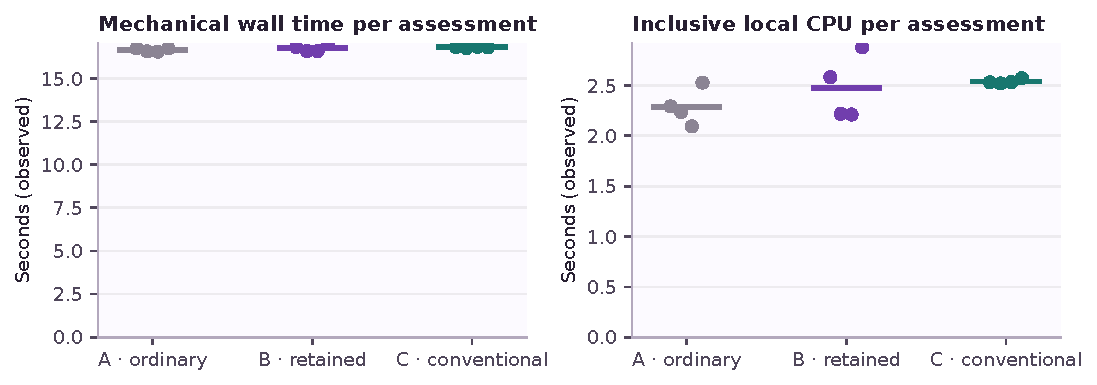
\includegraphics[width=\textwidth]{figures/production.pdf}
\caption{Executed evidence, without an assumed speed premium. Each point is an actual
arm/tuple observation. The retained producer removes an explicit finalization action, while the
mechanical runtimes show no established economic speed advantage.}
\end{figure}

The exact campaign records setup CPU of 19.894 seconds, inclusive delivery CPU of 29.198 seconds
and packet-packaging CPU of 0.056 seconds. These phase totals must not be added to nested
per-job diagnostics a second time. They exclude unmeasured authoring, discovery and human work.
The source freeze remains unchanged; 448 packet payload hashes were checked.
A clean relocated replay rebuilt two environments from offline wheels and reproduced the same
joint-1 semantic result through the unchanged B Workbench. It is verification of the original
mission, not an additional customer job.

\section{The strategic market, explicitly}
\subsection{Players, information, actions and timing}
The model is a behavioral agent-based repeated procurement game with strategic posted-price
responses. It is not a solved equilibrium. There is no Nash, convergence, optimal-policy or
market-clearing claim.

There are twelve heterogeneous project buyers, one studied enterprise, a competent human provider,
a competing AI service and each buyer's conventional DIY option. Deferral is always available.
The three enterprise arms are separate common-draw counterfactual worlds, not three firms bidding
simultaneously against each other. Each starts with equal resources, information and customer draws.
B and C can construct or adopt the same class of reusable asset; neither is forced to reinvent it.

Each of 52 weeks first resolves due collections and bills, then accrues overhead and upkeep,
evaluates investment, posts prices and processes fresh supported opportunities in keyed random
order. Delivery and attention capacities bind. Accepted work generates invoices; rejected work
retains its cost without acceptance revenue. Delayed feedback changes trust and can cause churn.
After week 52 a drain interval resolves contracted collections/refunds without generating new work.

Buyers know their own task value, effort cost, budget, available offers and past outcomes.
They do not observe true future quality. Providers see past sales and public prices, not future
draws or private buyer values. Available actions include choosing or deferring work, switching,
excluding a disappointing provider temporarily, adjusting a posted price, adopting an asset,
maintaining it, retaining reserves and stopping after insolvency.
Every firm has finite cash and capacity. The simulation's hypothetical competitor automation is
an explicitly assumed response, not technology constructed by this study.

\subsection{Buyer payoff and feasible choices}
For buyer \(i\), provider \(j\) and week \(t\), modeled expected surplus is
\begin{equation}
U_{ijt}=\hat q_{ijt}V_i-p_{jt}-w_i e_{ijt}
 -(1-\hat q_{ijt})L_i-d_{ijt}-s_{ijt}.
\label{eq:utility}
\end{equation}
Here \(V_i\) is expected useful task value, \(p\) the posted price, \(w e\) remaining customer effort,
\(L\) consequence of an error, \(d\) delay cost and \(s\) switching/integration cost.
The value prior is an assumed multiple of wage-equivalent task effort, not revealed willingness
to pay. Buyer-specific trust uses bounded Beta-style counts and delayed outcome feedback;
the finite component passes are not inserted as unbiased field-quality estimates.

An offer is unavailable when the buyer budget, provider capacity, financeability or temporary
exclusion prevents delivery. Offers weakly worse on quality, price, effort, delay and switching
cost, and strictly worse on at least one, are removed. Under deterministic choice the highest
strictly positive utility wins. An alternative logit rule samples only from positive-utility,
nondominated feasible offers plus deferral at utility zero. Thus a random taste shock cannot
make a strictly dominated offer win. This is a deliberate behavioral restriction, not a fitted
consumer-choice law.

A finite procurement allocation is committed on accepted invoices. Refunds/defaults do not restore
it, a conservative simplification. Each buyer has at most one new changed-input opportunity per week;
unsupported opportunities cannot generate an enterprise job. The assumed scope fraction and arrival
process do not extrapolate the experiment to the digital-work market.

\subsection{Competition and price responses}
The ordinary enterprise explores the declared \money{5}, \money{10}, \money{20}, \money{40} and
\money{80} targets using past conversion and a margin-weighted exploration score. This is a
finite-horizon heuristic, not competent optimization by definition. Fixed-target and
cost-pass-through policies already exist in the frozen core. A fixed target posts at least current
unit cost plus \money{1}; a low target can therefore produce different realized prices before and
after adoption.

The human provider can compress markup toward cost after poor sales. The AI competitor can
respond to sales or undercut within a floor; an adequately funded competitor can purchase its
assumed cost reduction after a declared date. Its cash, obligations, sales and automation action
are recorded. Alternative fixed and adverse strategies are tested. No provider receives unlimited
free improvements, and the conventional DIY option retains its customer's effort cost.

\section{Calibration: attributable anchors and unidentified quantities}
\begin{table}[H]
\centering\small
\caption{External evidence constrains the model without identifying the exact offering's price.
Sources were checked on 26 October 2026.}
\begin{tabularx}{\textwidth}{p{27mm}p{49mm}Y}
\toprule
Evidence & Attributable observation & Permitted interpretation and limitation\\
\midrule
BLS wages & May 2025 median developer \money{135,980}/year;
QA \money{104,300}/year \cite{blswages} &
Labor opportunity-cost anchor. Dividing by assumed 2,080 annual hours gives
\money{65.375} and \money{50.144}/hour; not a bill rate or task duration.\\
BLS compensation & June 2026 private wages \money{32.82}/hour;
total compensation \money{46.89}/hour \cite{blsecec} &
Benefits-loading sensitivity across occupations, not measured software-specific construction cost.\\
Historical contracts & Upwork Python typical \money{20}--\money{40}/hour;
median \money{30} \cite{upwork} &
A cheaper competent-human alternative. Worldwide historical platform summary, not a quote for this packet.\\
Conventional tools & Renovate community hosted tier has zero license price;
Dependabot creates update PRs \cite{renovate,dependabot} &
A strong incumbent with remaining setup, test and review effort. Zero license price is not zero total cost.\\
Advertised AI plans & Copilot Pro \money{10}/month; CodeRabbit Essentials
\money{30}/month or \money{24} annual-billed equivalent \cite{copilot,coderabbit} &
Alternative budget scale. Subscription prices are not complete-deliverable transactions or unlimited task capacity.\\
Maintenance practice & GOV.UK documents recurring dependency obligations and qualified automation \cite{govuk} &
Observed need for maintenance. Does not establish this study's buyer arrival rate or willingness to pay.\\
Adoption attitudes & Stack Overflow 2026 reports heterogeneous trust in AI output \cite{survey} &
Motivates competing trust models. Survey responses are not purchase probabilities or population weights.\\
\bottomrule
\end{tabularx}
\end{table}

The full source manifest has fifteen primary-source entries, each with what it supports and what
it does not. Advertised offers, historical transactions, public budgets, attitudes and actual
study purchases are distinct evidence classes. This study observes no completed purchase of its
exact offering. A primary empirical study of Dependabot compatibility scores motivates
consumer-specific evidence but cannot calibrate present commercial demand \cite{dependabotstudy}.

The reference scenario uses a \money{65.38} provider-hour anchor, \money{30} human-provider-hour
anchor and heterogeneous buyer-hour anchors of \money{30}, \money{50.14} and \money{65.38}.
Transporting wages to this task and combining these groups are assumptions. Task durations of
30/60/90 minutes, remaining review of eight minutes, a 1.25 usefulness multiplier, error loss,
trust priors, reliability and payment behavior are unidentified. No implicit conversion of an
AI researcher action into ten human minutes is made: zero, two, ten and thirty avoided minutes
are separately declared scenarios.

Default initial capital is \money{1,000}, reserve \money{200}, setup \money{50} and weekly overhead
\money{2}. The market-size convention is twelve projects, not an estimated total addressable
market. The default \money{0.25} compute/tool allowance is an assumption, not an invoice.
Full historical engineering cost is also unidentified. The illustrative four-hour case plus a
\money{100} authoring allowance gives \money{361.52}; it is neither a measured total nor an upper
bound. Failure/discovery shares allocate that total rather than adding a second copy.

The parameter manifest records every default and classification. Primary scenarios, later
exploration and stress inputs remain separate. Very weakly identified quantities may lie outside
every displayed range; apparent robustness inside the grid is not empirical identification.

\section{Exact-asset finance and accounting}
\subsection{Cash, accrued expense and economic outcome}
Every event is explicitly typed as simulated. For enterprise \(f\),
\begin{equation}
C_{t+1}=C_t+\mathrm{Collections}_t-\mathrm{CashPayments}_t,\qquad C_t\geq0.
\end{equation}
Bills accrue once and remain obligations until paid. A due bill that cannot be paid marks
insolvency and stops new delivery. Revenue is not earned by rejected work; accepted but
uncollected invoices remain separate from collected money. Defaults, refunds and delivery
failure costs are retained. Economic profit is recognized invoices net of defaults less every accrued cost,
including refunds and unpaid obligations. After the complete collection drain, recognized net
invoices equal gross collections. Seed capital is never revenue.

The unchanged \texttt{alpha-shadow-ledger/v1} arithmetic supplies the economic and liquidity
projections. Its native observed-collection category requires observed evidence. Therefore
observed collections remain exactly zero, while simulated collections enter only an explicitly
assumed-price projection with a \texttt{SIMULATED} wrapper. Refund adjustments are explicit,
and paid costs are not added again to the same accrued expense.

\subsection{Affordability and investment alternatives}
An adoption is eligible only if the forecast benefit after upkeep, anticipated price pass-through
and lost delivery during adoption exceeds its full prospective charge. The forecast uses only
trailing eight-week accepted enterprise sales, remaining productive weeks and a declared
discount. It cannot read future demand.

In addition, adoption cost must fit current cash net of obligations and reserves. The stricter
earned-funding mode also caps it by accumulated collected operating surplus excluding seed
resources and uncollected invoices. Precisely, with accrued costs \(E_t\), unpaid obligations \(O_t\),
reserve \(R\) and gross collections \(Y_t\), its available amount is
\[
F_t^{\rm earned}=\min(C_t-O_t-R,\ Y_t-E_t-R).
\]
This conservative policy also requires a reserve out of cumulative net earnings, even when initial
capital supplies liquidity. It is an eligibility rule, not an additional cost or a theorem that
smaller profits cannot finance adoption. Reserve sensitivity is available in the interface but
was not swept in the final diagnostic. Seed-funded adoption is separately labeled. Installation
takes at least one week, or the ceiling of adoption hours divided by available engineering
hours; successful installation pauses service and no asset use is permitted before availability.
The frozen failure branch charges the full adoption cost but treats a failed integration as
immediately detected, allowing ordinary delivery to resume without forced downtime. Planned
activation metadata is not evidence of failed-installation downtime; prolonged failures are not bounded by that stress.

The model records reconstruction cost and selects the cheaper public-method adoption route.
The enterprise can retain its incumbent, adopt that solution, maintain an adopted asset,
preserve funds or stop. B and C have equal access to the existing method. The same exact source identity appears in the investment record
and every later use.

\textbf{Full-history and prospective accounting answer different questions.}
Full-history accrues the assumed historical research bill at opening, funded from initial finite
capital or left as an insolvency obligation. Earnings cannot retroactively finance that past work.
The separately labeled adoption-only view charges future installation, verification and upkeep
while excluding sunk research. It cannot establish repayment of omitted history.
An explicit retrospective-cost-allocation stress is retained but never called historical
research affordability.

No second productive successor is supplied. The next-investment action remains retain reserves
unless a distinct constructed, tested and worthwhile asset exists. This is a substantive limit
on the claimed flywheel, not a missing bookkeeping entry.

\section{Prospective primary experiment and preserved failures}
The primary source, scenarios, seeds and claim criteria were frozen before execution and publicly
recorded \cite{marketfreeze}. Eighty-seven configurations crossed avoided minutes, historical
construction or adoption assumptions and two buyer rules, plus named stresses. Twenty-four
independent seeds (1001--1024) yielded 2,088 paired worlds and 6,264 enterprise histories.
Semantic random keys exclude arm names, so random-call order cannot create an artificial
B/C advantage.

\begin{resultbox}
\textbf{Primary result.} No world adopted the capability and no enterprise trajectory had
positive complete scenario profit. Under reference assumptions A loses \money{154};
B and C each lose \money{515.52}, including the declared \money{361.52} historical charge.
All three attract zero accepted enterprise sales in that reference condition.
\end{resultbox}

This does not demonstrate financeable improvement under the specified primary policies and assumptions.
It does not establish that every possible offering or competent pricing policy fails.
B/C tie exactly because their modeled effects, costs and random draws are equal.
The finite production observations justify avoiding an unsupported AGI ALPHA premium;
they do not empirically identify equal total construction cost.

\begin{figure}[H]
\centering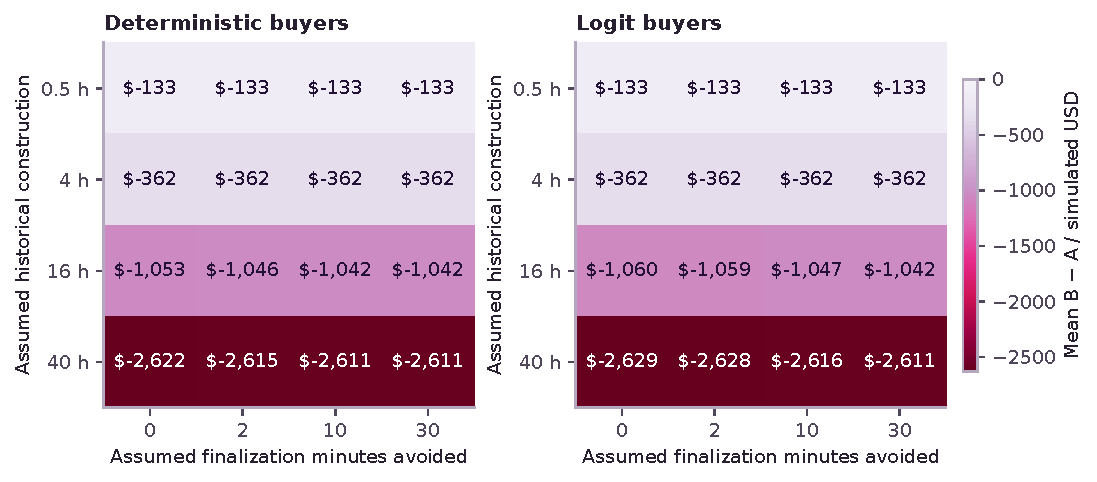
\includegraphics[width=\textwidth]{figures/primary.pdf}
\caption{Primary full-history grid: mean B-minus-A economic outcome in simulated USD.
Historical hours include the same declared authoring allowance. No cell adopts, so the
investment comparison retains the opening historical charge without a later operating saving.
Both buyer rules and all failures are preserved.}
\end{figure}

The primary stresses include no/low demand, cheap humans, cheap competing AI, price competition,
slow collections, dissatisfaction, switching barriers, quality shock, high upkeep, failed
integration, skeptical buyers, cash constraints and a free perfect conventional option.
These are adverse tests, not alternative favorable calibrations selected for publication.

\section{Exploration and pricing-policy diagnosis}
\subsection{Postprimary exploration with no replacement of the primary result}
A second protocol was designed and publicly frozen after inspecting the primary null
\cite{exploratoryfreeze}. It is explicitly exploratory. The same frozen core evaluated integration
costs of \money{0}/\money{10}/\money{50}, arrival probabilities .25/.5, avoided minutes
0/2/10/30, two buyer rules and four historical/prospective and earned/seed financing regimes.
Fourteen adverse corners added the declared stresses to a low-friction condition.
The 206 configurations used twelve new seeds (2001--2012), totaling 2,472 paired worlds.

Only six B worlds adopted, all under the seed-inclusive policy. Seventeen individual B worlds were profitable,
all in adoption-only accounting, and no configuration had positive mean B profit.
The sole configuration with positive mean B-minus-A difference produced \money{18.49}, with
a conditional normal-approximation 95\% Monte Carlo interval of
[\money{-15.17}, \money{52.16}]. Its mean B profit was \money{-103.83}.
This is not a robust profitable enterprise or financing from earned surplus.
The grid fractions are not estimates of real-world customer probabilities.

Direct payback also fails as a substitute for causal evaluation. In one adopted path, direct
net saving is \money{11.21}, but total B-minus-A outcome is \money{-48.78}.
A pause, different allocation or pricing response can consume a component-level saving.

\subsection{A concrete policy inadequacy}
An independent reviewer inspected existing histories without changing or running new scenarios.
In the low-friction, .5-arrival, ten-minute, deterministic adoption-earned slice, the original
enterprise posted \money{80} during 506 of 624 enterprise-weeks and won none of 2,167 offers at
that price. It posted \money{20} for 18 weeks and won 17 of 87 offers.
The margin-weighted optimism term can keep an unbought high price attractive in a finite
market with few observations. The earlier failures therefore mix market conditions with a poor
pricing heuristic.

This is a concrete reason for a final bounded policy diagnostic, publicly frozen before its outcomes \cite{policyfreeze}. It is not a reason to delete
earlier outcomes or select an undisclosed favorable model. The diagnostic uses the unchanged
core and all five already-declared fixed target prices, with the existing cost floor exposed.
It evaluates 160 configurations: two integration costs, two arrival rates, ten assumed avoided
minutes, both buyer rules and four funding/cost regimes, on the same twelve exploratory seeds.
The matched draws enable policy comparison; they are not independent confirmation after selection.
Every target, failure and actual posted-price range is retained.

% SPDX-License-Identifier: Apache-2.0
\subsection{A narrow prospective deployment region}
The final diagnostic completes 1,920 paired worlds. B adopts in 398, all under the seed-inclusive funding policy:
199 full-history and 199 adoption-only. No earned-funded path adopts.
Four of 160 conditions have positive mean B profit. Every one uses zero integration cost,
.5 arrival probability and adoption-only seed funding: the \money{10}/\money{20} targets under
deterministic/logit choice. Their mean profits are respectively \money{129.51},
\money{106.46}, \money{96.72} and \money{183.28}. No \money{10}-integration or .25-arrival
condition has positive mean B profit.

Twenty conditions have positive mean B-minus-A outcome, all adoption-only seed-funded;
fifteen have a positive lower conditional Monte Carlo bound. Across individual worlds, 82 B paths
are profitable: 66 adoption-only seed, 14 adoption-only earned with no adoption, and two
full-history seed paths. The two individually profitable full-history paths still perform worse
than their A counterparts. Across the diagnostic, 62 B worlds combine positive profit with positive incremental value,
all adoption-only seed-inclusive. Seventy-two direct-payback worlds nevertheless have negative
B-minus-A value. These counts do not estimate a real enterprise's success probability. No full-history condition has positive mean B profit or positive mean B-minus-A effect.

\begin{table}[H]
\centering\small
\caption{Preselected diagnostic slice: \money{20} target, zero integration, .5 work arrival,
ten assumed avoided minutes, logit, twelve reused seeds. A mean profit is \money{-1.69}
in all rows. Monetary values are simulated USD.}
\begin{tabularx}{\textwidth}{Yrrrr}
\toprule
Cost and funding basis & B mean profit & B--A mean & Adopted & Profitable\\
\midrule
Full history; earned & $-363.21$ & $-361.52$ & 0/12 & 0/12\\
Adoption only; earned & $-1.69$ & $0.00$ & 0/12 & 4/12\\
Full history; seed & $-178.24$ & $-176.55$ & 12/12 & 1/12\\
Adoption only; seed & $183.28$ & $184.97$ & 12/12 & 12/12\\
\bottomrule
\end{tabularx}
\end{table}

Prospective B profit ranges from \money{15.03} to \money{397.09}, with median
\money{122.65} and sample standard deviation \money{119.69}. Paired gains range
\money{62.31}--\money{314.62}, median \money{158.36}, standard deviation \money{78.06}.
With historical cost included, 11/12 B paths lose money: the range is
\money{-346.49}--\money{35.57}, median \money{-238.87}. Every paired investment effect
is negative in that full-history condition, from \money{-299.21} to \money{-46.90}.
These are realized model dispersions, not uncertainty bounds on real markets.

In the last row the mean-profit interval is [\money{115.56}, \money{251.00}], and the paired
increment interval is [\money{140.80}, \money{229.13}]. All twelve paths directly repay the
prospective adoption and upkeep. The \money{20} quote remains \money{20} before and after
adoption, so this slice does not depend on a hidden automatic price reduction.
At the \money{10} target, actual quotes fall from the \money{14.33} cost floor to \money{10}
after adoption; that channel is explicitly recorded.

\begin{figure}[H]
\centering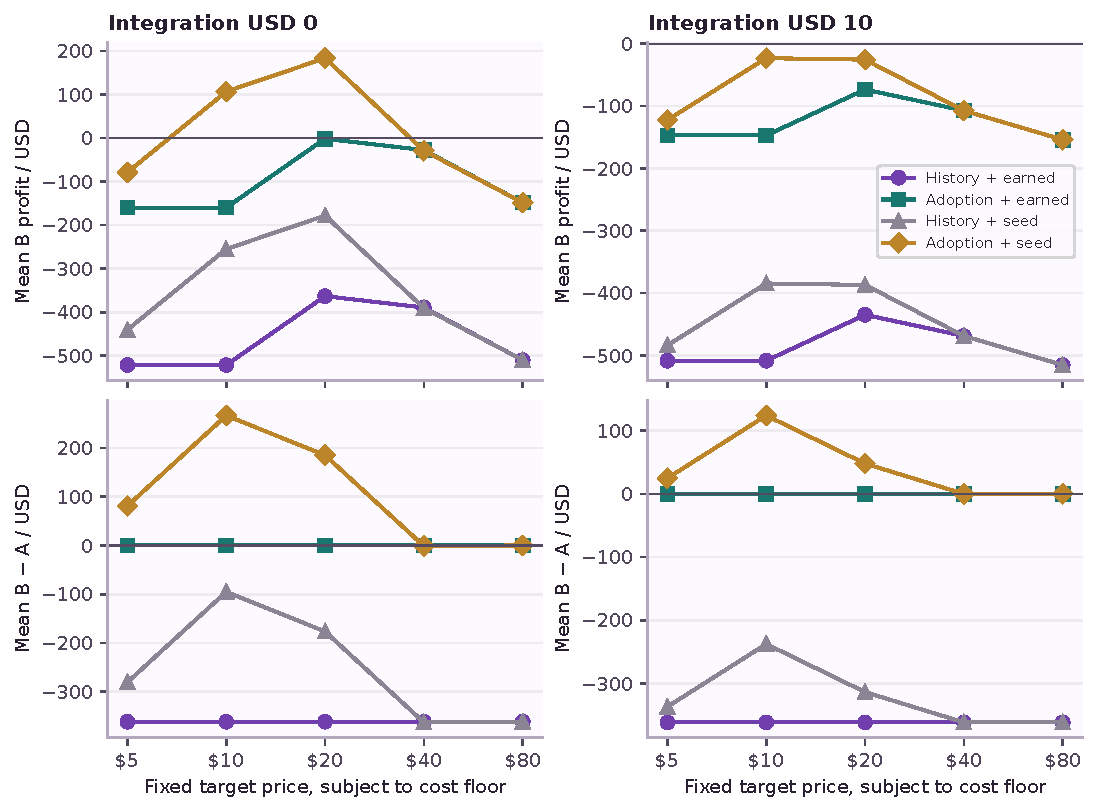
\includegraphics[width=\textwidth]{figures/policy.pdf}
\caption{All five target policies in the predeclared figure slice, including losing prices.
Top: mean B economic profit. Bottom: paired B-minus-A effect. Arrival .5, ten assumed avoided
minutes and logit are fixed. Adding \money{10} integration eliminates positive mean profit.
Full-history and prospective accounting are never pooled. Exact intervals and all 160
configurations appear in the companion table.}
\end{figure}

\subsection{One connected enterprise history}
The preselected seed 2001 illustrates deployment without selecting a winning trajectory after
the run. Under adoption-only seed funding it has 282 new-work opportunities, of which 213 fit
scope. The enterprise attempts 29, accepts 28 and rejects one; alternatives and deferral handle
the rest. At week 8, \money{745.37} is currently available after obligations and reserve.
The exact producer's \money{32.69} prospective adoption charge fits that cash, service pauses
one week and the asset becomes available at week 9. It is used on 17 subsequent modeled jobs.

The same enterprise collects \money{560}, incurs \money{437.35} total declared prospective
costs including a \money{20} refund, and finishes with \money{122.65} profit and
\money{1,122.65} cash. Adoption plus upkeep is \money{54.19}; direct avoided cost is
\money{190.75}. Its paired incremental gain is \money{136.56}. The AI competitor responds with
lower quotes and pays \money{200} for its declared automation at week 12. All these events are
simulated; the source-bound packet remains the actual production evidence.

The earned-surplus gate still reports \money{-77.35}, because this financing rule withholds a
\money{200} reserve from accumulated net earnings as well as checking liquidity.
Available cash and earned funding are deliberately different. The same path including
historical research finishes at \money{-238.87} profit and \money{-224.96} incremental value.
A visible cash balance therefore cannot be presented as historical cost repayment. Sixteen
other diagnostic paths end with positive earned availability after the reserve, but none has
a second constructed and tested asset to purchase.

\begin{figure}[H]
\centering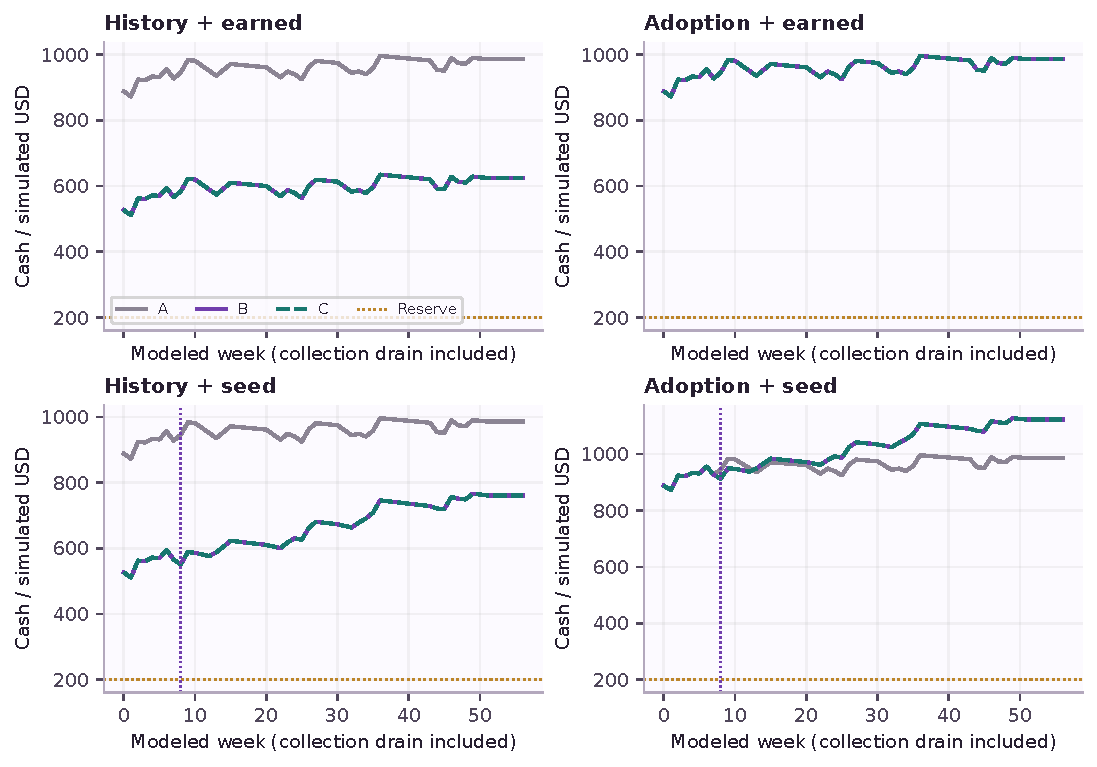
\includegraphics[width=\textwidth]{figures/history.pdf}
\caption{The same preselected seed across four accounting/funding regimes. B and C overlap.
Dotted vertical lines mark adoption; the horizontal line is the liquidity reserve.
Final collection weeks remain in the trace. No later hypothetical asset is purchased.}
\end{figure}

The narrow prospective region is a post-exploratory diagnostic on reused seeds. At this stage,
it has not been independently confirmed or stress-validated under every fixed-price interaction.
The earlier cheap-competitor, maintenance and quality stresses remain preserved, but their
heuristic-price outcomes cannot certify robustness of these new target policies.
A separately frozen fresh-seed extension follows below. It probes robustness of this selected
policy without identifying an optimal price or outside-market predictive performance.


\section{Viable regions, thresholds and what reverses the result}
\subsection{Demand has a ceiling as well as a supplier cost floor}
Let \(U^*_{it}=\max(0,\max_{j\ne E} U_{ijt})\) denote the buyer's best feasible alternative.
A deterministic enterprise purchase requires a price below
\begin{equation}
p^{\max}_{it}=\hat q_{iEt}V_i-w_i e_{iEt}
 -(1-\hat q_{iEt})L_i-d_{iEt}-s_{iEt}-U^*_{it},
\label{eq:ceiling}
\end{equation}
subject to capacity and budget. Equality can tie under the specified rule.
A retained capability can lower an affordable cost floor, while trust, usefulness, customer work
and competitors determine this ceiling. There need not be a profitable interval between them.

One exact primary replay illustrates the identity. At week 1, buyer 0 has an enterprise ceiling
of approximately \money{10.47}, while the reference policy posts \money{40}. In the zero-minute
scenario the same buyer purchases a \money{10} offer, with only about \money{0.47} utility
advantage. Another buyer's ceiling is approximately \money{-11.64}; even a free offer loses
because the modeled remaining work, risk and friction exceed the alternatives.
These are conditional utility calculations, not elicited willingness to pay.

\subsection{Repayment is path-dependent}
For a realized paired path, define \(K_{\rm charged}\) as the complete one-off capability expense
actually incurred under the declared accounting basis. The fixed-path threshold
\begin{equation}
K_{\max}^{\rm path}=\Delta_{BA}+K_{\rm charged}
\label{eq:threshold}
\end{equation}
is the maximum one-off cost consistent with nonnegative incremental value \emph{holding that
realized path fixed}. Maintenance, competition and forgone delivery remain inside \(\Delta_{BA}\).
This is an accounting diagnostic, not a global break-even theorem: changing cost can change
adoption eligibility, timing, pricing, sales and solvency. Unknown real costs remain unknown.

For an even simpler necessary saving calculation, ten avoided minutes at the wage anchor equal
about \money{10.90} per completed use before customer price pass-through, upkeep, failure and
foregone work. A \money{361.52} historical bill would require more than 33 such fully retained
savings even before those other charges. Zero measured human minutes would yield zero such
labor saving. This illustrates the sensitivity; it does not assert that the action really takes
ten minutes or that 34 buyers will appear.

\subsection{Most consequential uncertainties}
The result can reverse with the true finalization burden, full engineering/authoring cost,
arrival rate, buyer integration work, trust, quality under real use, competitive task prices
and pricing policy. Collection delay can make a positive-looking investment unaffordable.
Maintenance or a failed integration can erase direct savings. Cheaper AI and competent human
providers reduce the reservation-price ceiling. A free conventional workflow remains a credible
option when the customer's remaining effort is small.

The experiments vary market environments and impose quality shocks, but the four fresh technical
missions are related tuples of previously exposed libraries. They do not identify an independent
distribution of field production difficulty. All Monte Carlo intervals describe randomness
within one declared model; they exclude this larger model and parameter uncertainty.
No market size, adoption curve or global profitable equilibrium is inferred.

\section{Validation, demonstration and successive cycles}
The independent same-session review exercised 26 controls against the final frozen core:
cash reconstruction; binding budgets and reserves; accepted-only invoices; defaults and refunds;
zero demand; dominated offers; free perfect DIY; common random draws; B/C symmetry; failed
integration; and no investment or asset use before affordability/availability.
Earlier failed controls and their correction receipts remain in the companion.
Not every intermediate development source version was captured; those old failure logs are
evidence of the development process, not a claim of exact replay of every superseded version.

All original studied-enterprise histories were independently re-audited, including every bill,
invoice, cash event, investment and canonical projection. The reviewer is another agent in the
same session, not an organizationally external auditor. The final diagnostic receives the same
review. An output-only replay exposes all competitor invoices, bills and cash events without
changing any original returned field in 6,480 paired worlds. Its independent audit covers
38,880 competitor accounts. The bounded continuation separately audits all 9,216 enterprise
and 18,432 competitor histories; the pure funding view has synthetic and independent controls. An offline browser check exercises the actual bilingual interface, downloads exact packet
bytes, checks reference/control scenarios, verifies narrow layouts and rejects external network
requests. The demo executes the same frozen simulation arithmetic.

The English/French laboratory lets readers inspect four actual packet downloads, quality evidence,
CPU/wall records, unknown costs and source hashes, then change demand, review effort, integration,
pricing, collections, funding and cost basis. A/B/C outcomes remain side by side. A connected
history exposes buyer choices, competitors, invoices, collections, cash, obligations, adoption and
subsequent asset uses. Measured and simulated panels use separate labels.

The study follows the same modeled enterprise over time, rather than splicing successful
trajectories from unrelated firms. It does not demonstrate a second constructed productive asset.
The selected cache candidate was not economically justified by the observed burden; the importer
was an existing owner's work. Consequently, reserves can remain available without authorizing
a fictitious successor. Basic conditional commercial viability, historical investment repayment,
a second improvement cycle and self-acceleration remain distinct claims. Construction becoming
more effective across comparable fresh problems has not been established.

\section{Protocol, currency and authority boundaries}
All four repositories were inspected and pinned. The AGI ALPHA production engine, inherited
capability records, canonical ledger and existing publication coordination remain intact.
The Fleet execution hold is respected. The corrected public importer snapshot is exported inertly;
it creates no active proof, runtime authority or settlement.

The AGIJobs \(\$AGIALPHA\) routes and the Manager's USDC6 route remain separate verified code paths.
This model uses USD scenario units and invokes neither. It includes no token issuance,
appreciation, gross-transfer profit, distribution, buyback or holder rights.
There is no new credential, subscription, spending, customer outreach or deployed-contract change.
Successful local arithmetic does not confer financial or operational authority.

% SPDX-License-Identifier: Apache-2.0
\section{From deployment value to financeable succession}
\subsection{A bounded continuation with fresh seeds}
The user's continuation asks how far the narrow deployment result can extend. It does not
replace any original experiment. Before fresh outcomes, we declared a 128-condition extension,
24 new seeds (3001--3024), the same 52-week horizon, \money{1,000} initial capital and
\money{200} reserve, with no replenishment. The \money{20} target is inherited from the
identified diagnostic slice; this is an explicitly selected-policy exploratory extension,
not a new primary test or a search over prices. Its complete freeze was publicly recorded
before execution \cite{successionfreeze}.

The main 48-cell grid crosses integration costs \money{0}/\money{2.50}/\money{5}/\money{10},
work arrival .1/.25/.5, deterministic/logit buyers and full-history/adoption-only accounting.
Eighty adverse corners test weekly upkeep of \money{2}/\money{5}, collection delays of
6/13 weeks, cheaper AI, cheaper humans, undercutting, a quality shock, failed initial integration
and dissatisfaction. Each intervention is specified at zero/\money{5} integration, .5 arrival,
both buyer rules and both cost bases. The failed-integration corner means immediate detection with a full charge and no forced
downtime; it does not represent a prolonged failed installation. Other calibration and the
core economic rules stay unchanged.
No horizon extension or relaxation of buyer preferences is allowed after outcomes.

The research envelope limits the new market run to 120 wall and CPU seconds and sets an
18:10:33 UTC research cutoff. Discovery is capped at three burdens and fifteen minutes;
at most one justified prototype could use twenty minutes of implementation and six fresh
confirmation missions across three arms. Unfinished work must be labeled unfinished.
Publication and custody work are separately recorded.

\subsection{A source-of-funds view without invented money}
Initial external funding does not itself disqualify a Flywheel. The question is whether later
productive activity generates resources that can finance another worthwhile asset without
repeated injections. Three accounts are therefore kept separate: prospective deployment,
full historical return and funding provenance.

The original strict earned-funds policy remains unchanged. A second read-only attribution
view deducts one reserve in the liquidity bound. Let \(H_t^{\rm seed}\) be only a verified
historical research bill paid from opening seed before any collections; \(U_t\) is an outstanding
generated-resource earmark not already accrued as expense. Then
\begin{equation}
G_t=\max\!\left[0,\,
\min(C_t-O_t-R,\ Y_t-E_t+H_t^{\rm seed})-U_t\right].
\label{eq:generated}
\end{equation}
Here \(Y_t\) is collected revenue and \(E_t\) all accrued expenses. Setup, first adoption,
delivery, failed integration, upkeep and refunds remain inside \(E_t\). Historical research
stays charged once in cash and full-return profit; it is excluded only from the prospective
operating-generation recovery subtotal. Unpaid or later research is never added back.
An earmark reduces both the cash and generation bounds, and is released when its bill accrues.
No actual second-asset commitment exists, so \(U_t=0\) in this study.

This convention identifies a funding ceiling, not an extra cash balance or a transfer.
The adoption-only end-of-year seed-2001 example has \money{122.65} in generated resources under
Equation~\ref{eq:generated}, while its original strict metric remains \money{-77.35}.
Its \money{200} liquidity reserve is protected in both views. A sensitivity also requires
historical research recovery in the generation bound.

The new discovery itself has unknown authoring/inference and human monetary cost. Denote this
incremental unpriced cost \(D\geq0\); it is not silently reclassified into the old historical bill
or treated as zero. Before new decisions alter a path, available funds after that discovery are
bounded above by \(\max(0,G_t-D)\), and its economic return falls by its attributed \(D\).
For paired arms the fixed-path effect becomes
\(\Delta_{BA}^{\rm after}=\Delta_{BA}^{\rm before}-(D_B-D_A)\);
unidentified differential discovery costs do not automatically cancel.
Reported \(G_t\) is consequently \emph{before this unpriced discovery}, not an all-in investment
budget. The complete cost of any candidate would have to fit the remaining amount.

\begin{figure}[H]
\centering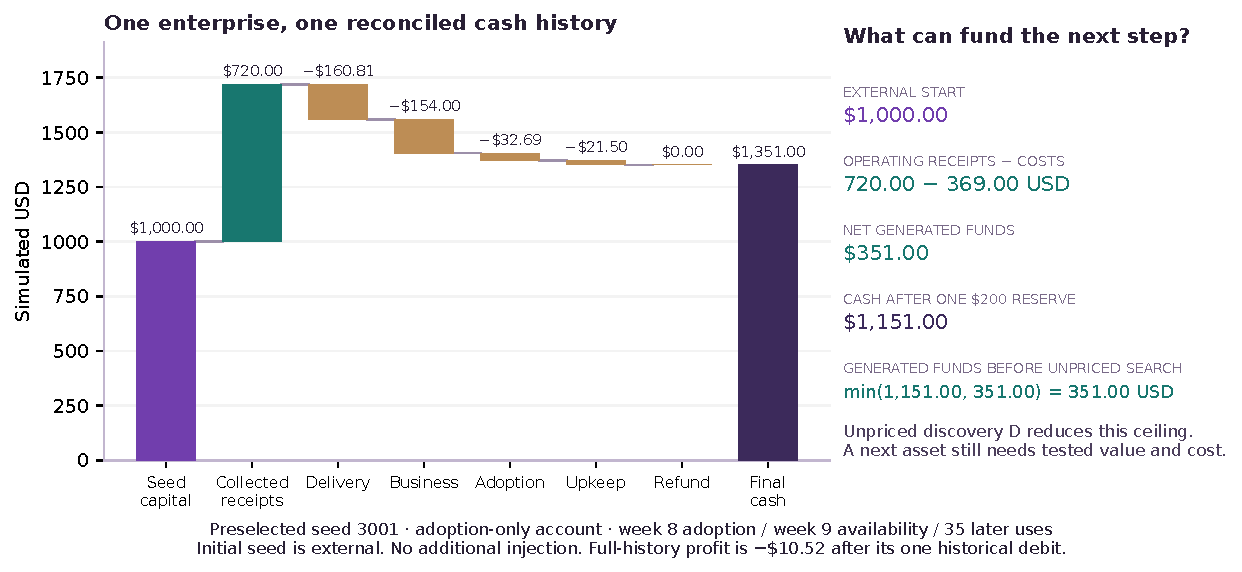
\includegraphics[width=\textwidth]{figures/finance.pdf}
\caption{Starting capital, productive collections, costs, reserves and the exact retained
investment in the connected fresh-seed path selected before extension outcomes. The provenance view exposes generated funds while
preserving the historical-return loss. The funding ceiling precedes the unpriced new discovery
cost \(D\); no hypothetical successor is purchased.}
\end{figure}

% SPDX-License-Identifier: Apache-2.0
\subsection{Fresh-seed outcomes and the viable region}
The registered extension completed all 3,072 paired worlds and 9,216 enterprise histories at
17:27:04 UTC, before the scientific cutoff. Its bounded invocation used 53.97 wall seconds and
60.52 child CPU seconds, below both 120-second limits. All 128 declared conditions are retained.
Every monetary result in this subsection precedes the unpriced incremental discovery cost \(D\).
This qualification applies to profit, paired effects and funding ceilings.

At the predeclared reference---\money{20}, zero integration, .5 arrival, logit choice and
seed-inclusive prospective adoption---mean B profit is \money{151.70}, with conditional
95\% Monte Carlo interval [\money{93.56}, \money{209.84}]. The paired gain is \money{173.67},
interval [\money{137.44}, \money{209.90}]. A's mean profit is \money{-21.97}. All 24 B paths
adopt, but three lose money. B profit ranges from \money{-140.33} to \money{474.62},
median \money{148.67}, sample standard deviation \money{145.32}. Paired gains range from
\money{0.31} to \money{338.21}, median \money{169.26}, standard deviation \money{90.55}.
Thus the fresh simulation retains a positive conditional mean deployment effect while exposing
downside absent from the original twelve-world slice.

Charging the same \money{361.52} historical allowance once changes reference mean B profit to
\money{-209.82} and its mean paired effect to \money{-187.85}; every reference paired effect
is then negative. Across all 64 full-history extension conditions, none has positive mean
B profit or positive mean B-minus-A. There are nevertheless 22 individual full-history worlds
with both a profit and a positive paired effect. These finite paths must not be erased, nor
treated as an estimated real-world success probability. Across the 64 prospective conditions,
18 have positive mean B profit and 47 have positive mean B-minus-A. B and C tie exactly throughout.

\begin{table}[H]
\centering\small
\caption{Fresh-seed main grid at .5 arrival. Prospective B profit and paired gain, before
unpriced discovery; 24 worlds per row. Parentheses give conditional 95\% Monte Carlo intervals.
Integration cost is buyer friction, not supplier revenue.}
\begin{tabularx}{\textwidth}{llYrr}
\toprule
Choice & Integration & Mean B profit (USD) & Mean B--A & Losses\\
\midrule
Logit & $0.00$ & $151.70\ (93.56,\ 209.84)$ & $173.67$ & 3/24\\
Logit & $2.50$ & $110.17\ (54.48,\ 165.85)$ & $147.42$ & 5/24\\
Logit & $5.00$ & $65.30\ (7.25,\ 123.36)$ & $114.24$ & 10/24\\
Logit & $10.00$ & $-23.69\ (-69.02,\ 21.64)$ & $59.71$ & 16/24\\
Deterministic & $0.00$ & $61.39\ (-54.65,\ 177.43)$ & $107.26$ & 13/24\\
Deterministic & $2.50$ & $-10.40\ (-90.35,\ 69.55)$ & $60.48$ & 16/24\\
Deterministic & $5.00$ & $-57.83\ (-111.96,\ -3.70)$ & $47.25$ & 18/24\\
Deterministic & $10.00$ & $-118.57\ (-144.41,\ -92.74)$ & $6.24$ & 23/24\\
\bottomrule
\end{tabularx}
\end{table}

In the logit grid, mean prospective profit changes sign between \money{5} and \money{10}
integration. The deterministic grid changes sign between \money{0} and \money{2.50}, and even
its zero-friction mean has a wide interval and a majority of losing paths. At .25 or .1 arrival,
no main-grid condition has positive mean B profit. These are sampled sign brackets, not fitted
exact break-even points, a universal monotonicity result or a license to extrapolate demand.
The assumed ten provider minutes remain essential unidentified input; fresh market seeds do not
turn an AI finalization-action count into measured human effort.

\begin{figure}[H]
\centering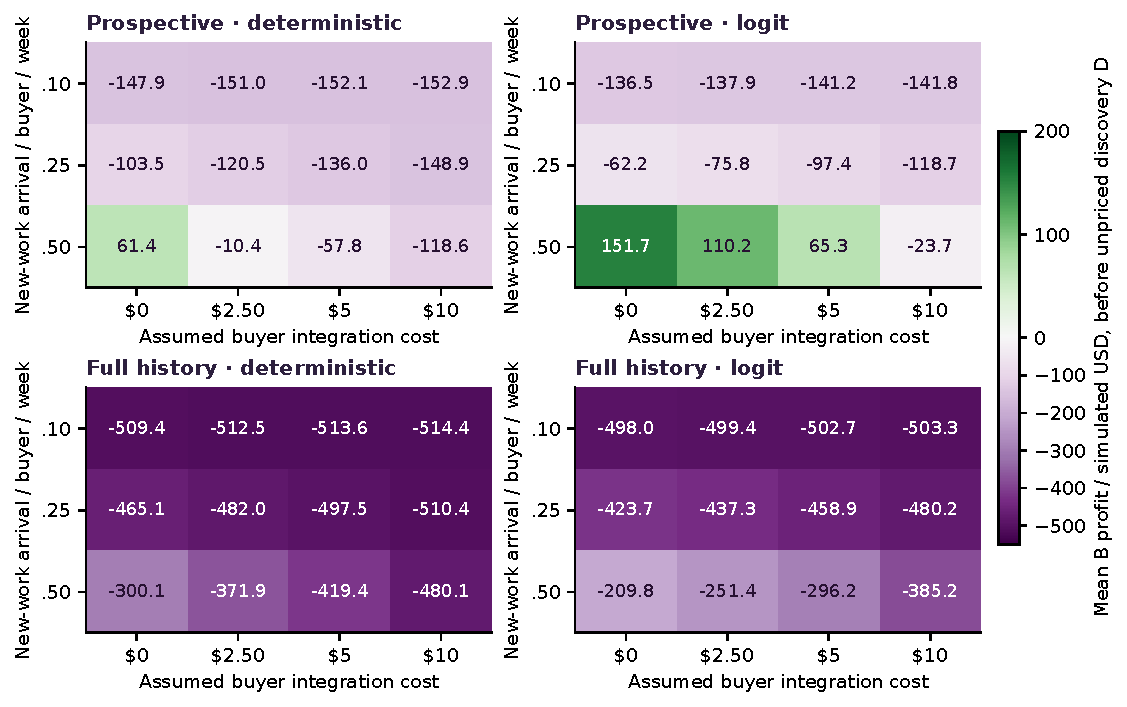
\includegraphics[width=\textwidth]{figures/succession-grid.pdf}
\caption{Every main extension cell, with the original horizon and capital. The prospective
region is sensitive to integration, recurrence and buyer-choice specification. Full-history
accounting remains separate. Values exclude the new unpriced discovery cost.}
\end{figure}

\begin{figure}[H]
\centering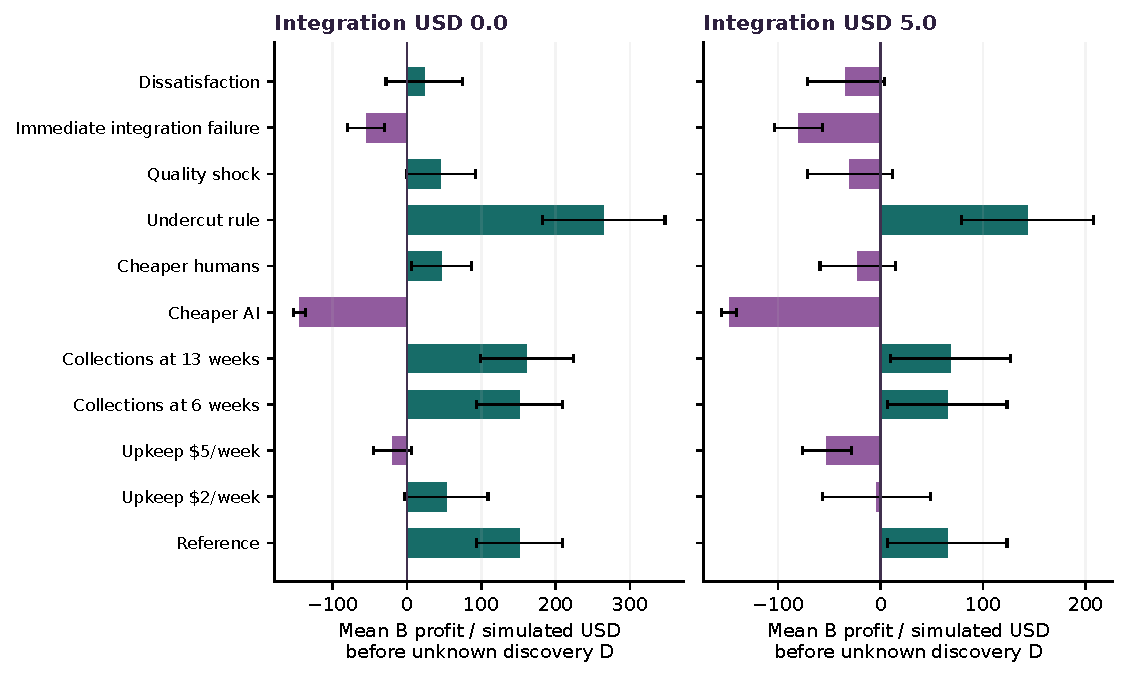
\includegraphics[width=\textwidth]{figures/succession-stress.pdf}
\caption{All ten predeclared perturbations and the reference for logit buyers at .5 arrival,
prospective accounting and zero/\money{5} integration. Intervals describe Monte Carlo variation,
not identified market parameters. A perturbation is not guaranteed to worsen outcomes under
every behavioral response. The complete table retains both buyer rules and both cost bases.}
\end{figure}

At zero integration, \money{2} weekly upkeep lowers mean B profit to \money{52.60};
\money{5} upkeep lowers it to \money{-19.85}. Cheaper AI removes deployment value:
mean profit is \money{-144.71} and mean B-minus-A is \money{-0.44}. Cheaper human provision
gives \money{46.31} mean profit, the quality shock \money{45.66}, and dissatisfaction
\money{23.40}; each becomes a negative mean at \money{5} integration.
Immediately detected failed integration produces \money{-54.66} profit and
\money{-32.69} incremental value at zero integration. It is a charged failure, not a free retry.

Collection timing alone does not necessarily reduce terminal profit when reserves cover the lag
and contracted receipts are drained. Six weeks reproduces the reference mean; thirteen weeks
gives \money{161.37}. Existing-event inspection finds 21/96 first buyer-choice divergences
across both integration levels and buyer rules; every one has unchanged quoted prices and a
human-provider cash gate that passes in the reference but binds under the longer delay.
For seed 3008 at week 35, a \money{67.50} delivery requirement fits \money{504.05} of reference
human-provider cash but exceeds \money{60.35} in the delayed path; that buyer switches to the
enterprise. No competitor insolvency occurs in these inspected cells.
Despite higher terminal mean B profit, the reference mean maximum during-service funding ceiling
falls from \money{153.04} to \money{69.68}. Payment timing can constrain succession before final
accounting catches up.

The undercut rule gives \money{264.54} mean profit because it sets the AI quote at \money{16},
whereas the adaptive reference reaches \money{7}--\money{17}. Fully 1,217 of 1,248 recorded
reference weekly quotes are below \money{16}; mean accepted AI jobs fall from 48.54 to 26.71,
and enterprise accepted jobs rise from 25.04 to 31.83. Undercutting the enterprise's \money{20}
is therefore weaker competition than many reference markdowns. These declared interventions
are not uniformly harsher conditions. The arithmetic inspection uses existing histories only;
it establishes a mechanism within this behavioral model, not a general benefit of delayed
payment, a favorable equilibrium or a real-world competitive advantage.

\subsection{Generated resources exist, but do not establish a second cycle}
The reference's mean terminal \(G\) is \money{162.29}, median \money{148.67}, range
\money{0}--\money{474.62}. Twenty-one of 24 paths have a positive terminal ceiling; twenty
have one during the productive year. This is a mean of nonnegative per-path ceilings, not
the mean profit of \money{151.70}. Charging historical research once does not automatically
erase operating generation: the cash bound still protects obligations and the reserve.
The stricter original prospective metric has mean \money{-48.30}.

The registered representative seed 3001 connects the entire sequence without selecting a
trajectory after outcomes. It has 321 changed-work opportunities, 249 supported, forty attempted
deliveries, 37 accepted and three rejected. Initial adoption costs \money{32.69} at week 8;
the exact first asset becomes available at week 9 and serves 35 later modeled jobs.
Gross invoices are \money{740}; \money{720} is collected and \money{20} defaults.
There are no refunds. Declared prospective costs total \money{369}: \money{154} business,
\money{160.81} delivery, \money{32.69} adoption and \money{21.50} upkeep.
Profit is \money{351}, cash \money{1,351}, and the paired gain \money{338.21}.
After the historical debit, profit is \money{-10.52}, cash \money{989.48} and paired gain
\money{-23.31}. The historical loss is visible even though the prospective operating-generation
ceiling is \money{351} under both cost bases.

This path first has a positive \(G\) at week 19; its maximum during the productive year is
\money{311}, followed by \money{351} after collections drain. The original strict metrics are
\money{151} prospective and \money{-210.52} full-history. These amounts cannot be spent before
they exist. No second asset is bought at any date.

For this path, a future investment could fit at most \(\max(0,351-D)\) dollars after the new
discovery, subject to its own timing, obligations and qualification. For the reference mean,
an attributed expected \(D_B\) reduces \money{151.70} of prospective profit dollar for dollar;
the paired benefit is also reduced by the differential cost \(D_B-D_A\). Neither cost is
identified. Accordingly, the study establishes a conditional supply of generated resources,
not all-in affordability or repayment of an unbuilt successor.


\subsection{The second-capability gate: no qualified purchase}
The bounded discovery examined three burdens in 321.8 elapsed seconds, not measured human labor.
Broader native application qualification is the most promising service direction: it could
extend a maintainer's component evidence into a fuller release decision. However, the current
61-case closure does not identify an authorized, reproducible broader contract, measured
remaining effort, complete cost bounds or a prospectively frozen fresh cohort.

Additional environment reuse already benefits all arms. The entire five-environment setup costs
19.894 CPU seconds, and changed tuples still require validation. No material extra attention
benefit is measured. Publication and accounting custody repairs are necessary research work,
but do not provide another productive capability for this component-assessment buyer.
The previously rejected baseline cache and existing importer owner's boundary remain intact.

The gate is therefore \textbf{NO-GO before construction}. There is no second implementation,
fresh second-asset confirmation, purchase, new customer job or claimed second-asset saving.
This does not say all future assets are worthless, and it does not erase the existing B/C
deployment value. The missing condition is a source-identified, worthwhile and tested next
asset whose complete cost fits generated funds after discovery, obligations and reserves.
Positive cash availability alone cannot supply that evidence.

\subsection{An evidence ladder}
\begin{table}[H]
\centering\small
\caption{Claims advance only as far as their evidence. Economic thresholds remain conditional
on declared scenarios and unidentified costs.}
\begin{tabularx}{\textwidth}{p{43mm}Y}
\toprule
Rung & Supported status\\
\midrule
Executed useful production & Established in the finite component scope: four fresh joint
questions, twelve complete assessments, actual reviewable decision packets.\\
Conditional deployment value & Positive within specified model conditions; preserved primary
failures and adverse outcomes remain visible. Original and fresh-seed results are separately labeled.\\
Full investment repayment & No tested full-history configuration has positive mean profit
or investment effect. Some individual paths do; actual all-in cost remains unknown.\\
Generated financing of a subsequent tested asset & Funding ceilings can be computed, but
no qualified second capability exists and its discovery cost is unpriced. A second cycle is not established.\\
Actual market receipts & Zero observed collections; no actual adoption is inferred from
simulated buyers or invoices.\\
Superior improvement process or self-acceleration & Not established. Conventional C ties B;
construction efficiency on comparable fresh problems has not been demonstrated.\\
\bottomrule
\end{tabularx}
\end{table}


\clearpage\section{Conclusion}
% SPDX-License-Identifier: Apache-2.0
The executed contribution is four new grouped dependency questions, twelve accepted finite-scope
assessments, exact replayable decision packets and a retained evidence-bound producer tested on
fresh tuples. Its automated finalization is real. A conventional builder matches its accepted
quality; human labor saved, all-in construction money and field reliability are not measured.

External evidence supplies labor anchors, practical conventional and AI alternatives, real
maintenance obligations and heterogeneous attitudes. Prices for this exact packet, recurring
purchase frequency, task value, human durations, integration effort and payment behavior remain
assumptions. All financial trajectories are simulations, and observed customer collections are zero.

The frozen primary result is negative. A later, explicitly exploratory pricing diagnostic finds
conditional value from deploying the existing asset. At the preselected \money{20} target,
zero integration, higher assumed recurrence and logit choice, mean prospective B profit is
\money{183.28} and mean B-minus-A is \money{184.97} across twelve worlds. Including the declared
historical cost gives \money{-178.24} mean B profit; eleven worlds lose money. Those results
remain unchanged.

The separately registered continuation tests that policy in 24 fresh worlds per condition.
At the same reference, prospective profit averages \money{151.70}, with three losing worlds,
and the paired gain averages \money{173.67}, before the new unpriced discovery cost.
Positive mean profit survives \money{2.50} and \money{5} integration under logit choice;
it fails at \money{10}, at the lower recurrence levels, and against the specified cheaper AI.
Deterministic buyers make the result less favorable. Upkeep, human competition, quality shocks
and dissatisfaction further constrain it. No tested full-history configuration in any campaign
has positive mean B profit or positive mean B-minus-A. This is not universal nonviability:
the extension includes 22 individual full-history worlds with both quantities positive.

Prospective deployment, full repayment and succession therefore have different answers.
The actual existing asset can be worth adopting from the current decision point. Full historical
repayment is not established. Some enterprises also generate resources that could contribute
to later investment without replenishing seed capital. In the preselected fresh path,
\money{720} of collections minus \money{369} of prospective costs leaves \money{351};
obligations and a \money{200} reserve fit within cash. The historical debit remains visible,
leaving full-history profit of \money{-10.52}. The new discovery cost \(D\) is unpriced,
so \money{351} is a ceiling before \(D\), not an all-in spendable commitment.

No second capability passed the bounded qualification gate. Broader native qualification needs
a defined contract and fresh evidence; additional environment reuse lacks a measured material
burden; research custody repairs are not another buyer-facing production asset.
The missing condition is a distinct tested improvement whose complete cost fits actual
then-available generated funds and whose incremental benefits justify that cost.
The experiment ends with no second construction or purchase. It does not infer a second cycle
from a balance, a scheduler or a diagram.

The most consequential uncertainties are competent-human finalization time, complete historical
and prospective engineering cost, buyer integration and review effort, recurring purchase
frequency, choice behavior and competing offers. The conventional tie does not erase useful
service or asset value; it limits the claim of a distinctive construction-method advantage.
Actual customer adoption, collected market revenue, earned financing of a subsequent tested
capability, self-acceleration and real-world self-financing remain unestablished.


\newpage
\appendix
\section{Evidence inventory and custody}
\small
\begin{longtable}{p{37mm}p{108mm}}
\toprule
Record & Identity and interpretation\\
\midrule
\endhead
Fresh production freeze &
\pathcode{2da7e8191eb2fb80adcd7d808d0494ab3247313e997607e7166e71c352ea7cee}.
144 exact source/input files; public before outcome.\\
Fresh campaign &
\pathcode{80ead6855a65d56dc2de4c84dc2063eefef92ae0d4c84421dfcd372b852f8084}.
Four missions, twelve assessments; zero actual customer collections.\\
Retained asset B &
\pathcode{0b4eb1ae2392176ff61ef91b7da0d13df3c6400ee0b3e317439238881adc182d}.
Exact source financed in every applicable model history.\\
Conventional asset C &
\pathcode{cd28579ecf72eba5bdfffa6b3b5483aaaa960322989d2a2369da5431062207ba}.
Strong reusable builder; its receipt checker is adopted by B.\\
Final market core &
\pathcode{52b7d83b57de1ca1cf43e444cedb3639193c91b2d6816f3ba86f9463dd904f27}.
Shared unchanged across all four campaigns and the demo.\\
Primary freeze &
\pathcode{7bbb0919ede3d4389d9eb36c23a7b775ec8093e40d51ac4da3f9c5714920406d}.
87 configurations; seeds 1001--1024.\\
Exploratory freeze &
\pathcode{7b4eb9450278cbe00400f442d964191a4bf15fd6726966955c03a0ebd22fa875}.
206 configurations; seeds 2001--2012.\\
Pricing diagnostic freeze &
\pathcode{640492e70fa9c4af9cd7093da24248b7b141cedb770941033a36e91f9094ea55}.
160 configurations; reused seeds 2001--2012.\\
Bounded continuation freeze &
\pathcode{e822d8a49f1d13f117543e17f628a8e230e672bc7d15b4d1bed4f5383f5bfd55}.
128 configurations; fresh seeds 3001--3024.\\
Funding provenance module &
\pathcode{7c017e77f26ca7c755e8fb832ec4e7eddfe241c758b769931e72fadedbb3e083}.
Read-only source-of-funds ceiling; discovery cost remains unknown.\\
Production closure &
\pathcode{031ac7a8098fc57267c552dda68963680291b3635a9132a4c9030025d04beb39}.
Manifest binds 1,498 selected files, 82,321,090 raw bytes.\\
Relocated production replay &
\pathcode{20bcd214f037b8e5884f34c407fe02de27a02f28aaa4d3cf40350e1801e619c0}.
Exact semantic agreement; zero additional unique missions.\\
\bottomrule
\end{longtable}
\normalsize
The inherited six-transition campaign, prior publications and failed custom candidate remain
distinct. Historical economic records are preserved with their disclosed custody gap; a missing
old upload receipt is not reconstructed as an observed original. The corrected importer is pinned
at commit \pathcode{269af6f9dd8d511fc387d0cecdff62a88ea96b02}; later owner edits are not silently
incorporated. The offline companion contains wheel licenses and source notices.

\section{Selected parameter and uncertainty ledger}
\begin{longtable}{p{37mm}p{37mm}p{70mm}}
\toprule
Quantity & Declared value or range & Identification / consequence\\
\midrule
\endhead
Field quality & Enterprise .95; human .97; DIY .95; AI .90 & Scenario values, not inferred from 4/4 or 6/6. Shocks and feedback affect choice and refunds.\\
New-work arrival & .25/week reference; 0/.1/.5 alternatives & Assumed per-project process. Recurring obligations establish a need class, not this frequency.\\
Supported share & .75 reference & Scope-transport assumption. Unsupported work cannot create delivery revenue.\\
Provider finalization & 0/2/10/30 minutes & Unknown human duration. The measured evidence is an explicit AI action count.\\
Customer effort & 8 minutes enterprise; 6 human; 15 AI & Assumed; unchanged by retained-asset admission. DIY uses .65 of task effort.\\
Capital and reserve & \money{1,000}; \money{200} & Equal starting resources across arms. Not observed funding or earned profit.\\
Historical construction & .5/4/16/40 hours plus \money{100} & Assumed whole-history allowance; no finite measured upper bound. Opening charge cannot be funded retroactively.\\
Prospective adoption & .5/4/16/40 hours & Existing solution may be adopted. Service pauses at least one week. No original R\&D repayment in adoption-only rows.\\
Maintenance & \money{0.50}/week reference; adverse variants & Scenario upkeep cost, charged only when relevant.\\
Collection & 2-week delay, .98 payment probability & Assumed; 13-week stress and defaults expose liquidity risk.\\
Mechanical requirement & 16.7994 wall / 2.5392 CPU seconds & Largest observed arm mean used as one-mission budget. Weekly machine availability remains assumed.\\
Service capacity & 4 enterprise jobs / 120 attention minutes per week & Scenario bottleneck, not a demonstrated deployment-scale benchmark.\\
Review and trust & Initial prior .90; skeptical share .25 & Behavioral assumptions; survey evidence does not identify these weights.\\
Pricing & Five targets, empirical or fixed-floor rules & Chosen strategy affects demand. Exhaustive target diagnostics are not optimized-policy confirmation.\\
\bottomrule
\end{longtable}
The machine-readable parameter manifest covers additional timing, budgets, correction,
refund, churn, competitor, forecasting and allocation variables. Full configuration snapshots
are embedded in every paired history, so published results never depend on an undocumented
default after the fact.

\section{Resource account and reproducible execution}
Actual phase receipts distinguish local CPU, wall time, input hashes, exit status and unknown
inference, authoring and human cost. Development failures, environment setup, verification,
packaging and recovery are retained. The canonical resource meter's inclusive process-child
CPU is used for phase accounting; nested task diagnostics are not summed again.
No all-in monetary profitability claim is possible from these receipts alone.

The primary simulator campaign took about 20.83 wall seconds and 23.29 inclusive CPU seconds;
the exploratory campaign about 30.24 and 33.37. These are local computational observations,
not cloud bills or authoring costs. The diagnostic uses 24.67 wall and 27.25 CPU seconds. The continuation bounded invocation
uses 53.97 wall and 60.52 CPU seconds. Exact receipts are included with each output.
The 150.73-wall/155.62-CPU-second competitor export is separately classified as same-world
custody replay, not a new economic campaign or a continuation research-budget charge.
Software environment: Python 3.12 Linux x86\_64 for frozen offline wheels, Node 24.22.1 for this
local research run. This is not a claim of the repository's separate Node 22.17.1 release gate.

From the complete companion root:
\begin{lstlisting}
# Validate the immutable production and financial records.
python3 production/audit_joint_results.py
node market/tests/test_market.mjs
node review/audit.mjs
node market/deployment-robustness/test-funding.mjs
python3 review/audit_outcomes.py market/results/primary-01 /tmp/primary-audit.json
# Repeat with exploratory or policy-diagnostic results and matching flags.
# See README for all exact commands; never overwrite a prior receipt.

# Frozen market runners reject an existing output directory.
node market/src/run.mjs --output /tmp/alpha-primary-replay
node market/exploratory/run.mjs --output /tmp/alpha-exploratory-replay
node market/policy-diagnostic/run.mjs --output /tmp/alpha-pricing-replay
node market/deployment-robustness/run.mjs --replay-registered --output /tmp/alpha-succession-replay

# Build the offline interface and publication.
python3 publication/build_demo.py
python3 publication/build_figures.py
python3 publication/build_succession_figures.py
python3 publication/build_finance_figure.py
cd publication
pdflatex -interaction=nonstopmode -halt-on-error paper.tex
pdflatex -interaction=nonstopmode -halt-on-error paper.tex
\end{lstlisting}
The continuation replay requires the original completed archive, verifies all fixed identities,
and reproduces the same registered worlds after the research cutoff; it creates no new evidence.
The root README supplies exact production instantiate/prepare/advance commands and path
relocation rules. Use fresh outputs. Embedded historical absolute paths are custody records,
not instructions to alter original locations. A full ZIP central-directory test, extraction
and per-file manifest comparison checks delivery closure. The bounded repository source PR
omits large histories/wheels and is clearly labeled; the complete companion provides them.

\section{Interpretive safeguards}
A larger positive outcome in an interactive user-selected scenario is a conditional illustration.
The reader has changed assumptions; it is not another independent market validation.
Normal-approximation intervals across twelve or twenty-four seeds summarize Monte Carlo
variability only. Closely related technical tuples, common scenario seeds and exhaustive grids
do not supply independent real-world replications. Multiple prices are all disclosed; a best
observed target is not described as a learned optimal strategy.

The product is deliberately scoped. It cannot certify all behavior, authentication, persistence,
security, platform compatibility or release readiness. A verification helper's passing tests
are not new buyer jobs. A positive supplier margin is not customer savings, and customer savings
are not supplier profit. A source-bound HOLD is not an execution authorization.

\newpage
\begin{thebibliography}{99}
\small
\bibitem{blswages} U.S. Bureau of Labor Statistics. \emph{Software Developers, Quality Assurance Analysts, and Testers}.
May 2025 wage statistics. Accessed 26 Oct 2026.
\url{https://www.bls.gov/ooh/computer-and-information-technology/software-developers.htm}.
\bibitem{blsecec} U.S. Bureau of Labor Statistics. \emph{Employer Costs for Employee Compensation---June 2026}.
Release 9 Sep 2026. \url{https://www.bls.gov/news.release/ecec.nr0.htm}.
\bibitem{upwork} Upwork. \emph{Python Developer Hourly Rates}.
Official indexed historical worldwide-contract summary; direct access returned 403.
\url{https://www.upwork.com/hire/python-developers/cost/}.
\bibitem{renovate} Mend. \emph{Mend Renovate Cloud Resource Tiers}.
\url{https://docs.mend.io/renovate/latest/mend-renovate-cloud-resource-tiers}.
\bibitem{dependabot} GitHub. \emph{Dependabot version updates}.
\url{https://docs.github.com/en/code-security/concepts/supply-chain-security/dependabot-version-updates}.
\bibitem{griffe} Griffe. \emph{Checking API compatibility}.
\url{https://mkdocstrings.github.io/griffe/guide/users/checking/}.
\bibitem{copilot} GitHub. \emph{Copilot plans and pricing}.
Current AI Credits plans. \url{https://github.com/features/copilot/plans}.
\bibitem{coderabbit} CodeRabbit. \emph{Plans and pricing}.
\url{https://docs.coderabbit.ai/management/plans}.
\bibitem{govuk} GOV.UK Publishing. \emph{Manage dependencies with Dependabot}.
Manual updated 11 Jun 2026.
\url{https://docs.publishing.service.gov.uk/manual/manage-dependencies.html}.
\bibitem{survey} Stack Overflow. \emph{2026 Developer Survey: AI trust}.
14,304 respondents; ODbL 1.0 attribution.
\url{https://survey.stackoverflow.co/2026/ai/data/ai-trust}.
\bibitem{dependabotstudy} N. Rombaut, F. R. Cogo, A. E. Hassan.
\emph{Leveraging the Crowd for Dependency Management: An Empirical Study on the Dependabot Compatibility Score}. 2024.
\url{https://arxiv.org/abs/2403.09012}.
\bibitem{starlette} Starlette maintainers and participants.
\emph{HTTPX 0.28 incompatibility with TestClient}, discussion 2770, Nov 2024.
\url{https://github.com/Kludex/starlette/discussions/2770}.
\bibitem{usefulwork} AGI ALPHA research contributors. \emph{Useful Work v2}.
Source and frozen companion, PR 4932.
\url{https://github.com/MontrealAI/AGI-Alpha-Agent-v0/pull/4932}.
\bibitem{nextupgrade} AGI ALPHA research contributors. \emph{The Next Upgrade}.
Preserved edition and ordered publication, PRs 4933--4934.
\url{https://github.com/MontrealAI/AGI-Alpha-Agent-v0/pull/4933}.
\bibitem{commercial} AGI ALPHA research contributors. \emph{Commercial study source}.
PR 4936. \url{https://github.com/MontrealAI/AGI-Alpha-Agent-v0/pull/4936}.
\bibitem{productionfreeze} AGI ALPHA issue 4850.
Prospective joint-tuple production freeze, comment 6421473941.
\url{https://github.com/MontrealAI/AGI-Alpha-Agent-v0/issues/4850#issuecomment-6421473941}.
\bibitem{marketfreeze} AGI ALPHA issue 4850.
Production outcome and prospective primary-market freeze, comment 6421724738.
\url{https://github.com/MontrealAI/AGI-Alpha-Agent-v0/issues/4850#issuecomment-6421724738}.
\bibitem{policyfreeze} AGI ALPHA issue 4850.
Prospective final pricing-policy diagnostic, comment 6422222209.
\url{https://github.com/MontrealAI/AGI-Alpha-Agent-v0/issues/4850#issuecomment-6422222209}.
\bibitem{exploratoryfreeze} AGI ALPHA issue 4850.
Primary failure and prospective exploratory freeze, comment 6421879271.
\url{https://github.com/MontrealAI/AGI-Alpha-Agent-v0/issues/4850#issuecomment-6421879271}.
\bibitem{successionfreeze} AGI ALPHA issue 4850.
Bounded deployment-robustness and succession extension, comment 6422814875.
\url{https://github.com/MontrealAI/AGI-Alpha-Agent-v0/issues/4850#issuecomment-6422814875}.
\end{thebibliography}
\end{document}
